\documentclass[12pt]{IEEEtran}

\usepackage{tikz}
\usepackage[utf8]{inputenc}
\usepackage{graphicx}
\usepackage{xcolor}
\usepackage{hyperref}
\usepackage{amsmath}
\usepackage{amsfonts}
\usepackage{amsthm}
\usepackage{amssymb}
\usepackage{mathrsfs}
\usepackage{graphicx}
\usepackage{adjustbox}
\usepackage{enumitem}
\usepackage[backend=biber,style=numeric]{biblatex}


%Chess Stuff
\usepackage[utf8]{inputenc}
\usepackage[english]{babel}
\usepackage{skak}
\usepackage{igo}

\definecolor{lightg}{rgb}{0.9,0.9,0.9}
\definecolor{lighta}{rgb}{0.7,0.7,0.7}

\title{How AI's Learn Board Games}
\author{Jason Miller}

\begin{document}
\maketitle

\tableofcontents

\section{Abstract}
This review will explore three different approaches that have been taken to optimize Chess and Go, one done by IBM's Watson Research Center and two done by Google's Deep Mind team. The ultimate goal is to understand the different techniques that were used to build the chess AI, \textit{Deep Blue}, and the two Go AIs, \textit{AlphaGo} and \textit{AlphaGo Zero}. We would also like to walk away with a better understanding of why some techniques work better than others.  

\section{Review}
\par Over the past few decades there has been a race for AI to surpass the decision making abilities of people. Calculators are able to do arithmetic better than people, and a computer can solve a Rubik's Cube faster than any person, but these aren't good metrics for decision making. Tasks like these are about one's ability to follow known steps to arrive at a singular conclusion. 

\par The gold standard for human supremacy over AI were the board games Chess and Go. Both are known for having such a magnitude of complexity that the best move has to be inspired instead of solved for. Using traditional techniques, solving for the best move would require billions of years of compute time. 

\par Over the past few decades these golds standards have been broken by AI. The first to fall was Chess, with Garry Kasparov losing to IBM's Deep Blue in a 1997 rematch. AI was able to surpass humans in Go when Google's AlphaGo won four games in a five game match against Lee Sedol in 2016. This victory was cemented with their improved iteration, AlphaGo Zero, which has won every match it has played against another person. We will explore the techniques that were developed to break these barriers and see the progression that has taken place over the past 30 years. 

\section{Deep Blue}
\par In a purely theoretical world, the way that we would find the best move is through a technique called min-max. The core assumption of min-max is that our opponent will make the best move possible on their turn. We can then find a move on our turn that leaves our opponent with the worst possible move out of the set of best moves they would make. This results in perfect play that leaves no gaps to be exploited. 

\scalebox{0.5}{
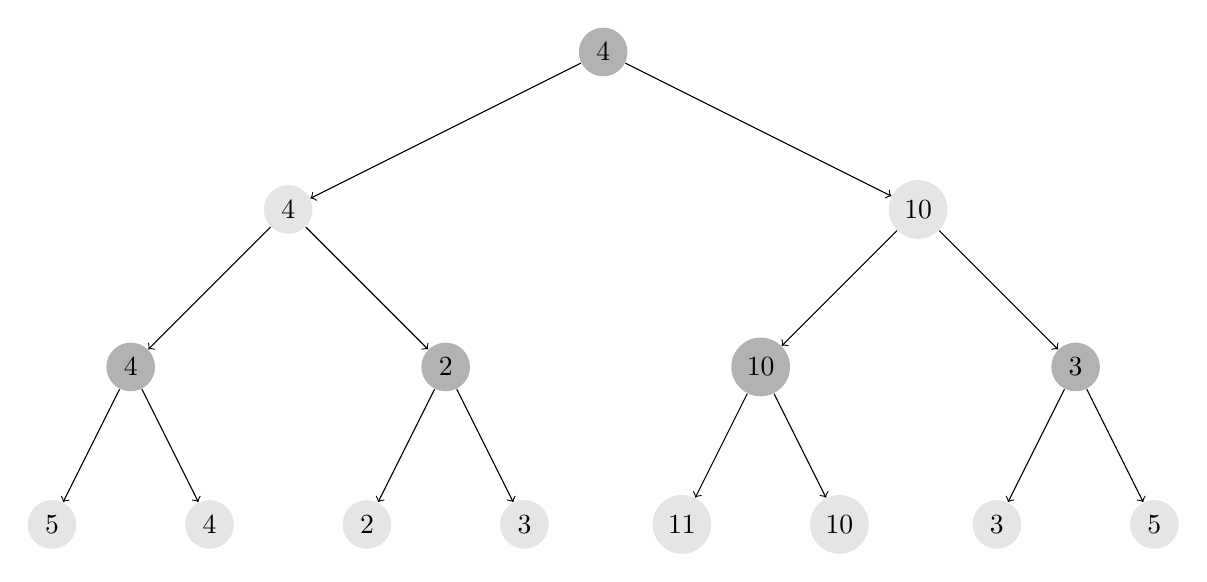
\begin{tikzpicture}
\node[circle,color=black, fill=lightg,minimum size=5pt] (5) at (8,4)  {11};
  \node[circle,color=black, fill=lighta,minimum size=5pt] (6) at (9,6)  {10};
  \node[circle,color=black, fill=lightg,minimum size=5pt] (7) at (10,4) {10};
  \node[circle,color=black, fill=lightg,minimum size=5pt] (4) at (11,8) {10};
  \node[circle,color=black, fill=lightg,minimum size=5pt] (1) at (12,4) {3};
  \node[circle,color=black, fill=lighta,minimum size=5pt] (2) at (13,6)  {3};
  \node[circle,color=black, fill=lightg,minimum size=5pt] (3) at (14,4)  {5};  
  \node[circle,color=black, fill=lighta,minimum size=5pt] (8) at (7,10)  {4};
  \node[circle,color=black, fill=lightg,minimum size=5pt] (9) at (4,4)  {2};
  \node[circle,color=black, fill=lighta,minimum size=5pt] (10) at (5,6) {2};
  \node[circle,color=black, fill=lightg,minimum size=5pt] (11) at (6,4)  {3};
  \node[circle,color=black, fill=lightg,minimum size=5pt] (12) at (3,8)  {4};
  \node[circle,color=black, fill=lightg,minimum size=5pt] (13) at (0,4) {5};
  \node[circle,color=black, fill=lighta,minimum size=5pt] (14) at (1,6)  {4};
  \node[circle,color=black, fill=lightg,minimum size=5pt] (15) at (2,4)  {4};
\draw[->] (8) to (4); 
\draw[->] (8) to (12); 
\draw[->] (4) to (2); 
\draw[->] (4) to (6); 
\draw[->] (2) to (1); 
\draw[->] (2) to (3); 
\draw[->] (6) to (5); 
\draw[->] (6) to (7);
\draw[->] (12) to (10); 
\draw[->] (12) to (14);
\draw[->] (10) to (9); 
\draw[->] (10) to (11);
\draw[->] (14) to (13); 
\draw[->] (14) to (15);    
\end{tikzpicture}}

\par In this diagram the dark gray nodes seek to minimize the outcome, while the light gray nodes seek to maximize the outcome. At each point the dark gray node will choose the smaller of its children and the light gray node will chose the smaller of the two children. Using these rules we can build the entire decision tree by only knowing the bottom layer. 

\par The key problem with min-max is that there is a bootstrapping issue. To find the best move on our turn requires that we can find our opponents best response to each move we can make. But to find our opponents best response we must find our best move for each possible board state two moves from now. This rapidly blows up until we are exploring every possible board that can ever exist. For chess this gives us about $2 * 10^{42}$ possible boards we need to consider each game, which is magnitudes more than the number of atoms on earth. 

\par The challenge that the IBM team was faced with was how to reduce the number of boards considered, without compromising on the quality of the move played. In the paper \textit{Deep Blue}, by Murray Campbell, A. Joseph Hoane Jr, and  Feng-hsiung Hsu it is revealed that they used two techniques to achieve this; an alpha-beta search and an evaluation function. 

\par Suppose that in our min-max search we found a particularly lethal response to a candidate move we are considering. We can pause our search of that candidate move until we are certain that all other moves we are considering have worse outcomes for us. This way we don't spend extra time exploring moves that present themselves as bad immediately. This approach is called alpha-beta search, and it limits our program to only exploring moves with merit and only considering dire moves in particularly devastating positions. 

\scalebox{0.5}{
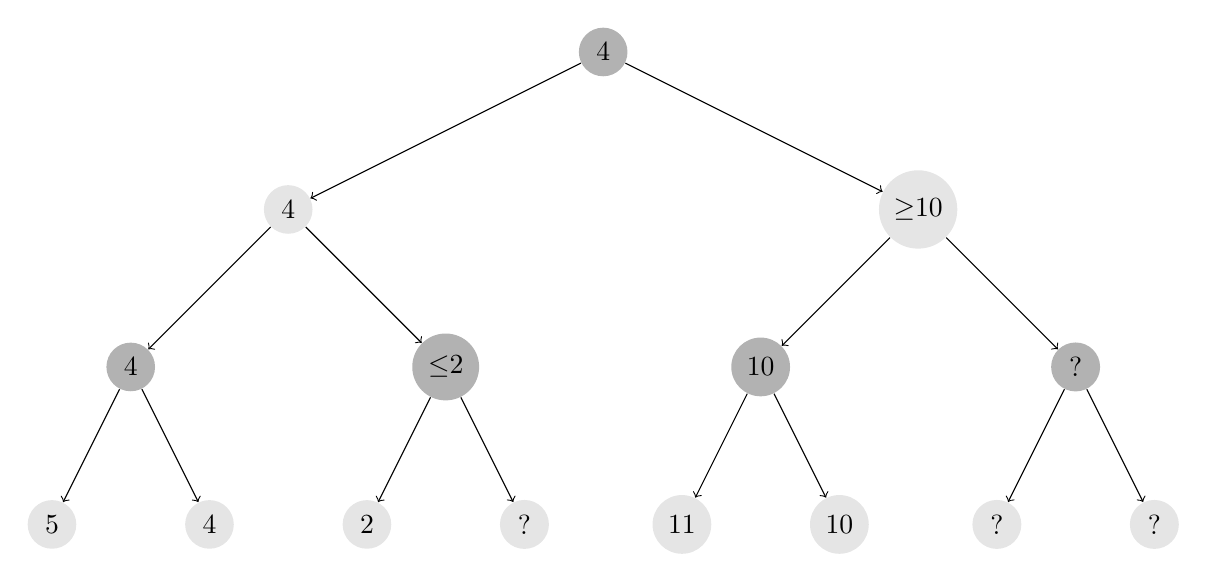
\begin{tikzpicture}
\node[circle,color=black, fill=lightg,minimum size=5pt] (5) at (8,4)  {11};
  \node[circle,color=black, fill=lighta,minimum size=5pt] (6) at (9,6)  {10};
  \node[circle,color=black, fill=lightg,minimum size=5pt] (7) at (10,4) {10};
  \node[circle,color=black, fill=lightg,minimum size=5pt] (4) at (11,8) {$\geq$10};
  \node[circle,color=black, fill=lightg,minimum size=5pt] (1) at (12,4) {?};
  \node[circle,color=black, fill=lighta,minimum size=5pt] (2) at (13,6)  {?};
  \node[circle,color=black, fill=lightg,minimum size=5pt] (3) at (14,4)  {?};  
  \node[circle,color=black, fill=lighta,minimum size=5pt] (8) at (7,10)  {4};
  \node[circle,color=black, fill=lightg,minimum size=5pt] (9) at (4,4)  {2};
  \node[circle,color=black, fill=lighta,minimum size=5pt] (10) at (5,6) {$\leq$2};
  \node[circle,color=black, fill=lightg,minimum size=5pt] (11) at (6,4)  {?};
  \node[circle,color=black, fill=lightg,minimum size=5pt] (12) at (3,8)  {4};
  \node[circle,color=black, fill=lightg,minimum size=5pt] (13) at (0,4) {5};
  \node[circle,color=black, fill=lighta,minimum size=5pt] (14) at (1,6)  {4};
  \node[circle,color=black, fill=lightg,minimum size=5pt] (15) at (2,4)  {4};
\draw[->] (8) to (4); 
\draw[->] (8) to (12); 
\draw[->] (4) to (2); 
\draw[->] (4) to (6); 
\draw[->] (2) to (1); 
\draw[->] (2) to (3); 
\draw[->] (6) to (5); 
\draw[->] (6) to (7);
\draw[->] (12) to (10); 
\draw[->] (12) to (14);
\draw[->] (10) to (9); 
\draw[->] (10) to (11);
\draw[->] (14) to (13); 
\draw[->] (14) to (15);    
\end{tikzpicture}}\\
\par In the diagram we don't explore most of the right side of the game tree. This is because light gray will have a payout of at least a 10, which makes dark gray prefer the entire left half of the game tree. Because of this, further exploration of the right side of the tree is not needed because it won't change the outcome of the decisions made. In the best case scenario this will square root the amount of nodes that need to be explored. 

\par But alpha-beta comes with a problem. For us to know that a move we are considering has a disastrous rebuttal, we must be able to know that the rebuttal is disastrous. If we are still playing out every possible game to know that it is a losing position, then little progress has been made in reducing the number of boards we must consider. This is where Deep Blue's evaluation function comes into play. This evaluation function takes a board, and does a weighted sum of the number of pieces each player has, as well as a few other calculations to get a estimate of who is ahead.\cite{DeepBlue} This way, bad moves can easily be discredited without having to play every possible board state to completion to demonstrate it. 

\par Some of the more advanced calculations that Deep Blue makes are things like if pieces are "pinned", is the King in danger, is a rook on the 7th row, are pieces trapped and so on. Deep Blue ended up with two evaluation functions; one simple, that only considered the easier to calculate board features, and a complex one, that added the advanced features. Both of these evaluation functions were coded into special CPUs as hardwired instructions to speed up compute time.\cite{DeepBlue} 

\par Murray Campbell, A. Joseph Hoane Jr, Feng-hsiung Hsu, go on to talk about how a suite of features that people consider when playing are embodied by the Deep Blue AI. For instance forcing moves, or moves where there is only a single good response, are handled well with the alpha beta search, which quickly discredits poor responses to allow compute time to be spent more meaningfully. Another common chess term is a piece being developed which means that the piece is active and useful. The freedom of movement of a piece and the tiles it threatens are embodied in the evaluation function, making sure they are accounted for whenever a move is considered. For instance, consider the following board position: 

\begin{center}
	\medskip
	\newgame
	\fenboard{2rr2k1/1p2qp1p/1pn1pp2/1N6/3P4/P6P/1P2QPP1/2RR2K1 w - - 0 20}
	\scalebox{1.2}{\showboard}
\end{center}

\par A simple evaluation of this board would show that black and white have the same amount of pieces on the board, 6 pawns, 2 rooks, a knight, a queen and a king. To see who is ahead we must look further into things like positioning. What we will notice is that black has a pair of stacked pawns on the $b$ and $f$ columns, as well as a exposed king. These factors are what Deep Blue considers when deciding who has advantage in a position. In fact, this is a position taken from game one of the 1996 game between Deep Blue and Garry Kasparov, with Deep Blue playing white and eventually winning the match. 

 Blending the alpha-beta search and this evaluation function, as well as dedicated hardware allows for extremely solid play. The evaluation function simplifying the game down to a manageable size and alpha-beta search efficiently finding optimal moved. Their combination allowed Deep Blue to take the $3\frac 12$ - $2 \frac 12$ victory over the best chess player in the world in 1997, Gary Kasparov, and advancing AI beyond what many thought possible. 

\section{AlphaGo}
\par Deep Blue's victory over Gary Kasparov was a resounding success for the progression of AI, but it had yet to conquer Go. Go is a game played on a $19 \times 19$ board, where the goal is to control more of the board than your opponent. Turns consist of a player placing a piece, called a stone, on the board. The more stones you have on the board and the more empty spaces you surround the more points you have, with the highest scoring player winning. The mechanism for conflict resolution is capturing. If a group of stones runs out of empty spaces adjacent to it, called liberties, it dies and is removed from the board. In the example below, black playing at the $X$ would capture the white stones. 


\gobansize{19}
\largegoban
\black{b3,c2,d3,d4,b4}
\white{c3,c4}
\gobansymbol{c5}{X}
\showgoban 
\cleargoban

\par Go has a larger game space than chess, with over $10^{172}$ possible boards that can be made. In addition, Go is known for being particularly difficult to build heuristics for, with solutions to fights often being counter intuitive, involving techniques like self sacrifice or rapidly switching direction of play at a whim. Additionally, because of shapes like kos and ladders, as well as it being a game of score, finding the correct move in a local situation requires considering the global status of the board. These factors all combine to create a game with such complexity that computers struggle to preform at even a basic level. 

\par With recent advancements in neural network, for tasks like image processing, the ability to train AI to process large data has improved dramatically. Google's Deep Mind team sought to build a Go AI by the name of AlphaGo by using neural networks to escape the difficulties of dealing with such complex board states. 

\par In IBM's approach to Deep Blue they overcame the two big challenges, how to efficiently search the space of all moves, and how to evaluate a board's position without playing to the end. Google took a similar approach by training two neural nets, a policy network and an evaluation network. The policy network's job is to try and predict the next move that will be played on the board, which it is able to do $\sim 57\%$ of the time on test data of real human games. The evaluation network tries to predict who is ahead based on the current board position. Both of these networks were trained using 30 million board positions from the online Go server KGS.\cite{AlphaGo} 

\par Below is a sample game from the show match between AlphaGo and Lee Sedol. The numbered stones are a move sequence that AlphaGo thinks is optimal play for both players. This sequence is used to inform AlphaGo's prediction of who is ahead. For this board, AlphaGo believes that black has $\sim$53\% chance to win. Move $1$ was a particular shock to the Go community. $1$ is called a shoulder hit because it approaches the white stone diagonally and from above it. Before AlphaGo shoulder hits were considered bad moves. They often directly reinforce the opponent's position with the follow up of $2$, without building territory directly. By being trained entirely on data, AlphaGo was able to recognize that the indirect value that the shoulder hit gives often outweighs the reinforcement that it gives its opponent, and the shoulder hit has become quite popular. 

\gobansize{19}
\black{c16,e16,j17,o16,q16,r15,p10,c6,d5,b4,c4,b3,d3,d2,k4,n4,o3,p4,q5}
\white{q14,r14,c13,d10,c7,b6,b5,c5,c3,d4,e4,f3,p3,q3,r4,r5,r6,q11}
\black[1]{p10}
\white[2]{p11}
\black[3]{o10}
\white[4]{p18}
\black[5]{n17}
\white[6]{r17}
\black[7]{s15}
\scalebox{0.5}{\showgoban} 
\cleargoban

\par To find the value of a single board position AlphaGo will use the evaluation function to guess the score, as well as the policy network to attempt to swiftly play the game to completion to get the final result. The idea being that the evaluation function will be able to identify high level structure while the policy network will see which player will likely win fights. Because this way to evaluate a board position is non deterministic, tools like alpha-beta search are not enough to explore the game tree. Instead AlphaGo opts for Monte Carlo Tree Search, which balances between searching moves that are unexplored and moves that are promising, or more commonly known as exploration vs exploitation.\cite{AlphaGo}

\par This combination of evaluation network and policy network allows AlphaGo to embrace both the territory scoring part of Go, as well as the combative capturing portion of the game. Various versions of AlphaGo were tried, with different levels of importance given to the evaluation network or the policy network when it came to choosing a move. Ultimately it was found that a balance of both networks was what allowed AlphaGo to preform best,\cite{AlphaGo} enabling it to beat Lee Sedol four games to one in a 2016 show match, conquering what was believed to be a insurmountable hurdle for AI. 

\section{AlphaGo Zero}
The original AlphaGo showed that AI had the capacity to beat top players, but the latest version, AlphaGo Zero, showed that AI has the ability to dominate top players. Google's AlphaGo Zero has not lost a single game to a human player ever. It was able to accomplish this through a complete reworking of how it was trained. 

\par For starters, AlphaGo Zero is trained without any data. It managed to learn the rules of the game entirely through self play and trained itself in a unsupervised way. Next, AlphaGo Zero does away with the evaluation and policy networks, opting instead for a singular all encompassing network. This network takes in only the board state, removing the additional information provided to the original AlphaGo in its evaluation function, and will produce an estimation for who is winning on the board. Finally, instead of the more exhaustive tree search that the original AlphaGo used, it instead uses a much simpler tree search that doesn't have the AI play out the game to completion, which was done with the old policy network.\cite{AlphaZero}

\par This simplified self play AI was able to vastly outperform the original AlphaGo. Within just 36 hours AlphaGo Zero was already stronger than its predecessor. Interestingly AlphaGo Zero is able to better predict the outcome of professional human games then AlphaGo, while having a worse ability to predict what the next move will be. This would be a strong indication that training AlphaGo on human games introduced a bias that, in the long run, decreased its performance. Even after just 72 hours, on one twelfths as much compute power, AlphaGo Zero won 100 out of 100 games in head to head matches with AlphaGo.\cite{AlphaZero}

\par With the creation of AlphaGo Zero, mankind's supremacy has been demonstrably destroyed. "Humankind has accumulated Go knowledge from millions of games played over thousands
of years, collectively distilled into patterns, proverbs and books. In the space of a few days, starting
tabula rasa, AlphaGo Zero was able to rediscover much of this Go knowledge, as well as novel
strategies that provide new insights into the oldest of games."\cite{AlphaZero}

\section{What Makes These AIs so Good?}
\par There is an example perfectly demonstrates why AI's approach to Go and other games are so successful. The first four moves of any Go game are typically one in each corner because corners are the easiest territory to take control of. Consider the following board positions: 

\gobansize{19}
\black{c3}

\white[1]{d4}
\black[2]{d3}
\white[3]{e4}
\black[4]{b5}
\white[5]{e3}
\black[6]{d6}
\white[7]{h3}
\scalebox{1}{\showgoban} 
\cleargoban

\par On this board black starts by claiming the corner with a 3-3 move and white approaches from the outside. The sequence that following is generally accepted to be optimal for both players following the 3-3. Notice that the amount of space in the bottom left of the board that is now black's territory. Now consider the following: 

\black{c4}
\white[1]{e4}
\black[2]{e3}
\white[3]{f3}
\black[4]{d3}
\white[5]{f4}
\black[6]{c7}
\white[7]{j3}
\scalebox{1}{\showgoban} 
\cleargoban

\par On this board black started by playing the 3-4 enclosure as their corner move. White then approaches again from the outside and the following optimal sequence happens. White's shape is the same in both sequences but black got slightly more territory in the corner by about 3 points. This would indicate that an initial corner move is better when it is closer to the center. Lets see if this trend continues:\\

\black{d4}
\white[1]{c3}
\black[2]{c4}
\white[3]{d3}
\black[4]{e3}
\white[5]{e2}
\black[6]{f3}
\white[7]{f2}
\black[8]{g3}
\white[9]{g2}
\scalebox{1}{\showgoban} 
\cleargoban

\par On this board black plays the 4-4 as their corner enclosure. This leaves enough space for white to jump into the corner with the 3-3 move and take all of the territory for themselves, giving black the entire outside. This dramatic shift in the direction of play would indicate that something special happened between moving from the 3-4 to the 4-4 corner enclosure. 

\par For hundreds of years people would play almost exclusively the 3-4 point and rejected the 4-4 point. Why would you play a move that doesn't guarantee any points? You aren't actually building value. This was until  a player by the name of Go Seigen came along and popularized the 4-4 point in the early 1900s. The philosophy behind the 4-4 point was: it would be dumb for white fight for the corner territory for a 3-3 or 3-4 enclosure because there are so few points. Likewise it would be dumb for white to try to take the outside when black plays the 4-4 enclosure, because the corner territory is so profitable. The key insight being that there is a balance between the tangible value that the corner territory gives, and the intangible value that owning the outside has. The 3-4 is the farthest move from the corner that has a slight preference for the inside and the 4-4 point is the closest move to the corner that has a slight preference for the outside. Both of these moves bookend a mystical optimal distance from the corner that balances the value of the inside and the outside perfectly. Because of this both should be considered as valid moves and are essentially two sides of the same coin. 

\section{Conclusion}
Though our hopes of competing against these AIs has been quashed, there is still much to be learned from them. Chess and Go are games with millennia of human study. To analyze how it is that deep learning was able to solve Chess and Go will give us insight into how AIs approach other tasks in less studied fields. The way that these AI learn the game of Go, and the challenges they had, might just reveal why self driving cars can crash, or why image recognition fails on certain objects, or even why hiring AIs discriminate against minority candidates. Further research should be undertaken to explore the interdisciplinary applications of AI's approach to Chess and Go. 

\begin{thebibliography}{1} 
\bibitem{DeepBlue}
Murray Campbell, A. Joseph Hoane Jr., Feng-hsiung Hsu. “Deep Blue” 2002. [Online]. Available: https://core.ac.uk/display/82416379?utm\_source=pdf\&utm\_medium=banner\&utm\_campaign=pdf-decoration-v1 [Accessed: 09-Nov-2021]. 

\bibitem{AlphaGo}
David Silver et al. “Mastering the game of Go with deep neural networks and tree search,” 28-Jan-2016. [Online]. Available: https://storage.googleapis.com/deepmind-media/alphago/AlphaGoNaturePaper.pdf [Accessed: 09-Nov-2021]. 

\bibitem{AlphaZero}
David Silver et al. “Mastering the Game of Go without Human Knowledge,” 19-Oct-2017. [Online]. Available: https://discovery.ucl.ac.uk/id/eprint/10045895/1/agz\_unformatted\_nature.pdf [Accessed: 09-Nov-2021]

\bibitem{ELF}
Yuandong Tian . “ELF OpenGo: An Analysis and Open Reimplementation of AlphaZero” 11-Jun-2019. [Online]. Available: https://research.fb.com/publications/elf-opengo-an-analysis-and-open-reimplementation-of-alphazero/ [Accessed: 09-Nov-2021]

\bibitem{WhyItWorks}
Tim Wheeler. “AlphaGo Zero - How and Why it Works” 2-Nov-2017. [Online]. Available: http://tim.hibal.org/blog/alpha-zero-how-and-why-it-works/ [Accessed: 09-Nov-2021]


\end{thebibliography}


\end{document}